% Created 2021-12-19 Sun 14:32
\documentclass[9pt, b5paper]{article}
\usepackage[UTF8]{ctex}
\usepackage{xltxtra}
\usepackage{bera}
\usepackage[T1]{fontenc}
\usepackage[scaled]{beraserif}
\usepackage[scaled]{berasans}
\usepackage[scaled]{beramono}
\usepackage{graphicx}
\usepackage{xcolor}
\usepackage{multirow}
\usepackage{multicol}
\usepackage{float}
\usepackage{textcomp}
\usepackage{geometry}
\geometry{left=1.2cm,right=1.2cm,top=1.5cm,bottom=1.2cm}
\usepackage{algorithm}
\usepackage{algorithmic}
\usepackage{latexsym}
\usepackage{natbib}
\usepackage{minted}
\newminted{common-lisp}{fontsize=ootnotesize}
\usepackage[xetex,colorlinks=true,CJKbookmarks=true,linkcolor=blue,urlcolor=blue,menucolor=blue]{hyperref}
\author{deepwaterooo}
\date{\today}
\title{Android Study Plan}
\hypersetup{
  pdfkeywords={},
  pdfsubject={},
  pdfcreator={Emacs 27.1 (Org mode 8.2.7c)}}
\begin{document}

\maketitle
\tableofcontents


\section{View相关}
\label{sec-1}

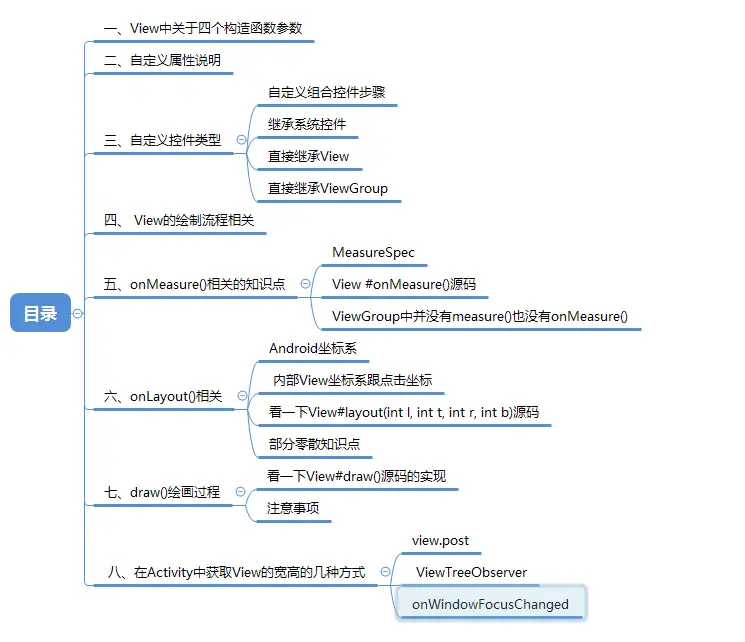
\includegraphics[width=.9\linewidth]{./pic/viewas.png}

\subsection{自定义View}
\label{sec-1-1}
\subsubsection{一、View中关于四个构造函数参数}
\label{sec-1-1-1}
\begin{itemize}
\item 自定义View中View的构造函数有四个
\end{itemize}
\begin{minted}[frame=lines,fontsize=\scriptsize,linenos=false]{java}
// 主要是在java代码中生命一个View时所调用,没有任何参数,一个空的View对象
public ChildrenView(Context context) {
    super(context);
}
// 在布局文件中使用该自定义view的时候会调用到,一般会调用到该方法
public ChildrenView(Context context, AttributeSet attrs) { // AttributeSet from .xml设置
    this(context, attrs,0);
}

// 如果你不需要View随着主题变化而变化,则上面两个构造函数就可以了
// 下面两个是与主题相关的构造函数
public ChildrenView(Context context, AttributeSet attrs, int defStyleAttr) {
    this(context, attrs, defStyleAttr, 0);
}
public ChildrenView(Context context, AttributeSet attrs, int defStyleAttr, int defStyleRes) {
    super(context, attrs, defStyleAttr, defStyleRes);
}
\end{minted}
\begin{itemize}
\item 构造函数的传入参数说明
\begin{itemize}
\item context:上下文
\item AttributeSet attrs:从xml中定义的参数
\item intdefStyleAttr:主题中优先级最高的属性
\item intdefStyleRes: 优先级次之的内置于View的style(这里就是自定义View设置样式的地方)
\end{itemize}
\item 多个地方定义属性,优先级排序 Xml直接定义 > xml中style引用 > defStyleAttr>defStyleRes > theme直接定义
\end{itemize}
\subsection{二、.xml中的自定义属性}
\label{sec-1-2}
\begin{itemize}
\item 基本类型包括: integer, boolean, color, string, float, dimension, enum, flags, fraction, reference
\item 基本类型略过,其它相对重要一点儿的
\end{itemize}
\subsubsection{color :引用颜色}
\label{sec-1-2-1}
\subsubsection{dimension: 引用字体大小}
\label{sec-1-2-2}
\begin{itemize}
\item 定义
\begin{minted}[frame=lines,fontsize=\scriptsize,linenos=false]{xml}
<attr name = "text_size" format = "dimension" />
\end{minted}
\item 使用:
\end{itemize}
\begin{minted}[frame=lines,fontsize=\scriptsize,linenos=false]{xml}
<app:text_size = "28sp"  />
<app:text_size = "@android:dimen/app_icon_size" />
\end{minted}
\subsubsection{enum:枚举值}
\label{sec-1-2-3}
\begin{itemize}
\item 定义
\begin{minted}[frame=lines,fontsize=\scriptsize,linenos=false]{xml}
<attr name="orientation">
  <enum name="horizontal" value="0" />
  <enum name="vertical" value="1" />
</attr>
\end{minted}
\item 使用:
\begin{minted}[frame=lines,fontsize=\scriptsize,linenos=false]{xml}
<app:orientation = "vertical" />
\end{minted}
\end{itemize}
\subsubsection{flags:标志 (位或运行) 主要作用=可以多个值}
\label{sec-1-2-4}
\begin{itemize}
\item 定义
\begin{minted}[frame=lines,fontsize=\scriptsize,linenos=false]{xml}
<attr name="gravity">
  <flag name="top" value="0x01" />
  <flag name="bottom" value="0x02" />
  <flag name="left" value="0x04" />
  <flag name="right" value="0x08" />
  <flag name="center_vertical" value="0x16" />
</attr>
\end{minted}
\item 使用
\begin{minted}[frame=lines,fontsize=\scriptsize,linenos=false]{xml}
<app:gravity = Top|left />
\end{minted}
\end{itemize}
\subsubsection{fraction:百分数:}
\label{sec-1-2-5}
\begin{itemize}
\item 定义:
\begin{minted}[frame=lines,fontsize=\scriptsize,linenos=false]{xml}
<attr name = "transparency" format = "fraction" />
\end{minted}
\item 使用:
\begin{minted}[frame=lines,fontsize=\scriptsize,linenos=false]{xml}
<app:transparency = "80%"  />
\end{minted}
\end{itemize}
\subsubsection{reference:参考/引用某一资源ID}
\label{sec-1-2-6}
\begin{itemize}
\item 定义:
\begin{minted}[frame=lines,fontsize=\scriptsize,linenos=false]{xml}
<attr name="leftIcon" format="reference" />
\end{minted}
\item 使用:
\begin{minted}[frame=lines,fontsize=\scriptsize,linenos=false]{xml}
<app:leftIcon = "@drawable/图片ID" />
\end{minted}
\end{itemize}
\subsubsection{混合类型:属性定义时指定多种类型值}
\label{sec-1-2-7}
\begin{itemize}
\item 属性定义
\begin{minted}[frame=lines,fontsize=\scriptsize,linenos=false]{xml}
<attr name = "background" format = "reference|color" />
\end{minted}
\item 使用
\begin{minted}[frame=lines,fontsize=\scriptsize,linenos=false]{xml}
<android:background = "@drawable/图片ID"  />
<android:background = "#FFFFFF"  />
\end{minted}
\end{itemize}
\subsection{三、自定义控件类型}
\label{sec-1-3}

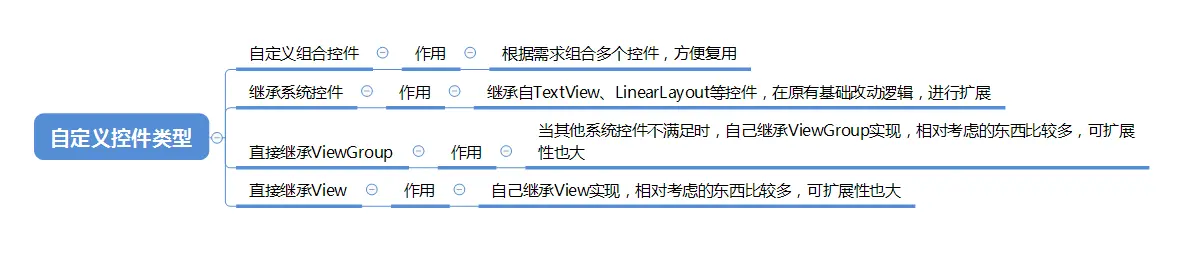
\includegraphics[width=.9\linewidth]{./pic/selfviews.png}

\subsubsection{自定义组合控件步骤}
\label{sec-1-3-1}
\begin{enumerate}
\item 1. 自定义属性
\label{sec-1-3-1-1}
\begin{itemize}
\item 在res/values目录下的attrs.xml文件中
\end{itemize}
\begin{minted}[frame=lines,fontsize=\scriptsize,linenos=false]{xml}
<resources>
  <declare-styleable name="CustomView">
    <attr name="leftIcon" format="reference" />
    <attr name="state" format="boolean"/>
    <attr name="name" format="string"/>
  </declare-styleable>
</resources>
\end{minted}
\item 2. 布局中使用自定义属性
\label{sec-1-3-1-2}
\begin{itemize}
\item 在布局中使用
\end{itemize}
\begin{minted}[frame=lines,fontsize=\scriptsize,linenos=false]{xml}
<com.myapplication.view.CustomView
    android:layout_width="wrap_content"
    android:layout_height="wrap_content"
    app:leftIcon="@mipmap/ic_temp"
    app:name="温度"
    app:state="false" />
\end{minted}
\item 3. view的构造函数获取自定义属性
\label{sec-1-3-1-3}
\begin{minted}[frame=lines,fontsize=\scriptsize,linenos=false]{kotlin}
class DigitalCustomView : LinearLayout {
    constructor(context: Context) : super(context)
    constructor(context: Context, attrs: AttributeSet?) : super(context, attrs) {
    LayoutInflater.from(context).inflate(R.layout.view_custom, this)
        var ta = context.obtainStyledAttributes(attrs, R.styleable.CustomView)
        mIcon = ta.getResourceId(R.styleable.CustomView_leftIcon, -1) //左图像
        mState = ta.getBoolean(R.styleable.DigitalCustomView_state, false)
        mName = ta.getString(R.styleable.CustomView_name)
        ta.recycle()
        initView()
    }
}
\end{minted}
\begin{itemize}
\item 上面给出大致的代码 记得获取context.obtainStyledAttributes(attrs, R.styleable.CustomView)最后要调用ta.recycle()利用对象池回收ta加以复用
\end{itemize}
\end{enumerate}
\subsubsection{继承系统控件}
\label{sec-1-3-2}
\begin{itemize}
\item 就是继承系统已经提供好给我们的控件例如TextView、LinearLayout等,分为View类型或者ViewGroup类型的两种。主要根据业务需求进行实现,实现重写的空间也很大 主要看需求。
\item 比如需求 :在文字后面加个颜色背景
\item 根据需要一般这种情况下我们是希望可以复用系统的onMeaseur和onLayout流程.直接复写onDraw方法
\end{itemize}
\begin{minted}[frame=lines,fontsize=\scriptsize,linenos=false]{kotlin}
class Practice02BeforeOnDrawView : AppCompatTextView {
    internal var paint = Paint(Paint.ANTI_ALIAS_FLAG)
    internal var bounds = RectF()
    constructor(context: Context) : super(context) {}
    constructor(context: Context, attrs: AttributeSet?) : super(context, attrs) {}
    constructor(context: Context, attrs: AttributeSet?, defStyleAttr: Int) : super(context, attrs, defStyleAttr) {}
    init {
        paint.color = Color.parseColor("#FFC107")
    }
    override fun onDraw(canvas: Canvas) {
        // 把下面的绘制代码移到 super.onDraw() 的上面,就可以让原主体内容盖住你的绘制代码了
        // (或者你也可以把 super.onDraw() 移到这段代码的下面)
        val layout = layout
        bounds.left = layout.getLineLeft(1)
        bounds.right = layout.getLineRight(1)
        bounds.top = layout.getLineTop(1).toFloat()
        bounds.bottom = layout.getLineBottom(1).toFloat()
        //绘制方形背景
        canvas.drawRect(bounds, paint)
        super.onDraw(canvas)
    }
}
\end{minted}
\begin{itemize}
\item 这里会涉及到画笔Paint()、画布canvas、路径Path、绘画顺序等的一些知识点,后面再详细说明
\end{itemize}
\subsubsection{直接继承View}
\label{sec-1-3-3}
\begin{itemize}
\item 这种就是类似TextView等,不需要去轮询子View,只需要根据自己的需求重写onMeasure()、onLayout()、onDraw()等方法便可以,要注意点就是记得Padding等值要记得加入运算
\end{itemize}
\begin{minted}[frame=lines,fontsize=\scriptsize,linenos=false]{kotlin}
private int getCalculateSize(int defaultSize, int measureSpec) {
    int finallSize = defaultSize;
    int mode = MeasureSpec.getMode(measureSpec);
    int size = MeasureSpec.getSize(measureSpec);
    //  根据模式对
    switch (mode) {
        case MeasureSpec.EXACTLY: 
            break;
        case MeasureSpec.AT_MOST: 
            break;
        case MeasureSpec.UNSPECIFIED: 
            break;
    }
    return finallSize;
}
@Override
protected void onMeasure(int widthMeasureSpec, int heightMeasureSpec) {
    super.onMeasure(widthMeasureSpec, heightMeasureSpec);
    int width = getCalculateSize(120, widthMeasureSpec);
    int height = getCalculateSize(120, heightMeasureSpec);
    setMeasuredDimension(width, height);
}
@Override
protected void onDraw(Canvas canvas) { // 画一个圆
    // 调用父View的onDraw函数,因为View这个类帮我们实现了一些基本的而绘制功能,比如绘制背景颜色、背景图片等
    super.onDraw(canvas);
    int r = getMeasuredWidth() / 2;
    // 圆心的横坐标为当前的View的左边起始位置+半径
    int centerX = getLeft() + r;
    // 圆心的纵坐标为当前的View的顶部起始位置+半径
    int centerY = getTop() + r;
    Paint paint = new Paint();
    paint.setColor(Color.RED);
    canvas.drawCircle(centerX, centerY, r, paint);
}
\end{minted}
\subsubsection{直接继承ViewGroup}
\label{sec-1-3-4}
\begin{itemize}
\item 类似实现LinearLayout等,可以去看那一下LinearLayout的实现 基本的你可能要重写onMeasure()、onLayout()、onDraw()方法,这块很多问题要处理包括轮训childView的测量值以及模式进行大小逻辑计算等,这个篇幅过大后期加多个文章写详细的
\item 这里写个简单的需求,模仿LinearLayout的垂直布局
\end{itemize}
\begin{minted}[frame=lines,fontsize=\scriptsize,linenos=false]{kotlin}
class CustomViewGroup :ViewGroup{
    constructor(context:Context):super(context)
    constructor(context: Context,attrs:AttributeSet):super(context,attrs){
        // 可获取自定义的属性等
    }
    override fun onMeasure(widthMeasureSpec: Int, heightMeasureSpec: Int) {
        super.onMeasure(widthMeasureSpec, heightMeasureSpec)
        // 将所有的子View进行测量,这会触发每个子View的onMeasure函数
        measureChildren(widthMeasureSpec, heightMeasureSpec)
        val widthMode = MeasureSpec.getMode(widthMeasureSpec)
        val widthSize = MeasureSpec.getSize(widthMeasureSpec)
        val heightMode = MeasureSpec.getMode(heightMeasureSpec)
        val heightSize = MeasureSpec.getSize(heightMeasureSpec)
        val childCount = childCount
        if (childCount == 0) {
            // 没有子View的情况
            setMeasuredDimension(0, 0)
        } else {
            // 如果宽高都是包裹内容
            if (widthMode == MeasureSpec.AT_MOST && heightMode == MeasureSpec.AT_MOST) {
                // 我们将高度设置为所有子View的高度相加,宽度设为子View中最大的宽度
                val height = getTotalHeight()
                val width = getMaxChildWidth()
                setMeasuredDimension(width, height)
            } else if (heightMode == MeasureSpec.AT_MOST) {
                // 如果只有高度是包裹内容
                // 宽度设置为ViewGroup自己的测量宽度,高度设置为所有子View的高度总和
                setMeasuredDimension(widthSize, getTotalHeight())
            } else if (widthMode == MeasureSpec.AT_MOST) {// 如果只有宽度是包裹内容
            // 宽度设置为子View中宽度最大的值,高度设置为ViewGroup自己的测量值
            setMeasuredDimension(getMaxChildWidth(), heightSize)
        }
    }
    // 获取子View中宽度最大的值
    private fun getMaxChildWidth(): Int {
        val childCount = childCount
        var maxWidth = 0
        for (i in 0 until childCount) {
            val childView = getChildAt(i)
            if (childView.measuredWidth > maxWidth)
            maxWidth = childView.measuredWidth
        }
        return maxWidth
    }
    // 将所有子View的高度相加
    private fun getTotalHeight(): Int {
        val childCount = childCount
        var height = 0
        for (i in 0 until childCount) {
            val childView = getChildAt(i)
            height += childView.measuredHeight
        }
        return height
    }
}
override fun onLayout(changed: Boolean, l: Int, t: Int, r: Int, b: Int) {
    val count = childCount
    var currentHeight = t
    for (i in 0 until count) {
        val child = getChildAt(i)
        val h = child.measuredHeight
        val w = child.measuredWidth
        child.layout(l, currentHeight, l + w, currentHeight + h) // 摆放子view
        currentHeight += h
    }
}
\end{minted}
\begin{itemize}
\item 主要两点 先 measureChildren()轮训遍历子View获取宽高,并根据测量模式逻辑计算最后所有的控件的所需宽高,最后setMeasuredDimension()保存一下 \#\#\#四、 View的绘制流程相关 最基本的三个相关函数 measure() ->layout()->draw()
\end{itemize}

\subsection{四、onMeasure()相关的知识点}
\label{sec-1-4}

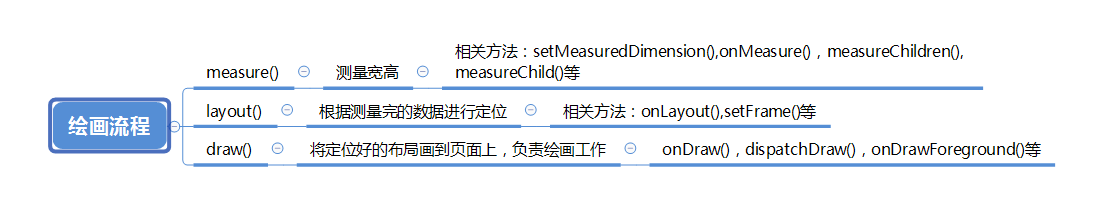
\includegraphics[width=.9\linewidth]{./pic/onmeasure.png}

\subsubsection{1. MeasureSpec}
\label{sec-1-4-1}
\begin{itemize}
\item MeasureSpec是View的内部类,它封装了一个View的尺寸,在onMeasure()当中会根据这个MeasureSpec的值来确定View的宽高。
\item MeasureSpec 的数据是int类型,有32位。 高两位表示模式,后面30位表示大小size。
\item 则MeasureSpec = mode+size 三种模式分别为:EXACTLY, AT$_{\text{MOST}}$, UNSPECIFIED
\begin{itemize}
\item EXACTLY: (match$_{\text{parent或者}}$ 精确数据值)精确模式,对应的数值就是MeasureSpec当中的size
\item AT$_{\text{MOST}}$:(wrap$_{\text{content}}$)最大值模式,View的尺寸有一个最大值,View不超过MeasureSpec当中的Size值
\item UNSPECIFIED:(一般系统使用)无限制模式,View设置多大就给他多大
\end{itemize}
\end{itemize}
\begin{minted}[frame=lines,fontsize=\scriptsize,linenos=false]{kotlin}
// 获取测量模式
val widthMode = MeasureSpec.getMode(widthMeasureSpec)
// 获取测量大小 
val widthSize = MeasureSpec.getSize(widthMeasureSpec)
// 通过Mode和Size构造MeasureSpec
val measureSpec = MeasureSpec.makeMeasureSpec(size, mode);
\end{minted}
\subsubsection{2. View \#onMeasure()源码}
\label{sec-1-4-2}
\begin{minted}[frame=lines,fontsize=\scriptsize,linenos=false]{java}
protected void onMeasure(int widthMeasureSpec, int heightMeasureSpec) {
    setMeasuredDimension(getDefaultSize(getSuggestedMinimumWidth(), widthMeasureSpec),
                         getDefaultSize(getSuggestedMinimumHeight(), heightMeasureSpec));
}
protected int getSuggestedMinimumWidth() {
    return (mBackground == null) ? mMinWidth : max(mMinWidth, mBackground.getMinimumWidth());
}
protected final void setMeasuredDimension(int measuredWidth, int measuredHeight) {
    boolean optical = isLayoutModeOptical(this);
    if (optical != isLayoutModeOptical(mParent)) {
        Insets insets = getOpticalInsets();
        int opticalWidth  = insets.left + insets.right;
        int opticalHeight = insets.top  + insets.bottom;
        measuredWidth  += optical ? opticalWidth  : -opticalWidth;
        measuredHeight += optical ? opticalHeight : -opticalHeight;
    }
    setMeasuredDimensionRaw(measuredWidth, measuredHeight);
}
public static int getDefaultSize(int size, int measureSpec) {
    int result = size;
    int specMode = MeasureSpec.getMode(measureSpec);
    int specSize = MeasureSpec.getSize(measureSpec);
    switch (specMode) {
    case MeasureSpec.UNSPECIFIED:
        result = size;
        break;
    case MeasureSpec.AT_MOST:
    case MeasureSpec.EXACTLY:
        result = specSize;
        break;
    }
    return result;
}
private void setMeasuredDimensionRaw(int measuredWidth, int measuredHeight) {
    mMeasuredWidth = measuredWidth;
    mMeasuredHeight = measuredHeight;
    mPrivateFlags |= PFLAG_MEASURED_DIMENSION_SET;
}
\end{minted}
\begin{itemize}
\item setMeasuredDimension(int measuredWidth, int measuredHeight) :用来设置View的宽高,在我们自定义View保存宽高也会要用到。
\item getSuggestedMinimumWidth():当View没有设置背景时,默认大小就是mMinWidth,这个值对应Android:minWidth属性,如果没有设置时默认为0. 如果有设置背景,则默认大小为mMinWidth和mBackground.getMinimumWidth()当中的较大值。
\item getDefaultSize(int size, int measureSpec):用来获取View默认的宽高,在getDefaultSize()中对MeasureSpec.AT$_{\text{MOST}}$,MeasureSpec.EXACTLY两个的处理是一样的,我们自定义View的时候 要对两种模式进行处理。
\end{itemize}
\subsubsection{3. ViewGroup中并没有measure()也没有onMeasure()}
\label{sec-1-4-3}
\begin{itemize}
\item 因为ViewGroup除了测量自身的宽高,还需要测量各个子View的宽高,不同的布局测量方式不同 (例如 LinearLayout跟RelativeLayout等布局),所以直接交由继承者根据自己的需要去复写。但是里面因为子View的测量是相对固定的,所以里面已经提供了基本的measureChildren()以及measureChild()来帮助我们对子View进行测量 这个可以看一下我另一篇文章:LinearLayout \# onMeasure()LinearLayout onMeasure源码阅读
\end{itemize}

\subsection{五、onLayout()相关}
\label{sec-1-5}
View.java的onLayout方法是空实现:因为子View的位置,是由其父控件的onLayout方法来确定的。
onLayout(int l, int t, int r, int b)中的参数l、t、r、b都是相对于其父 控件的位置。
自身的mLeft, mTop, mRight, mBottom都是相对于父控件的位置。
\subsubsection{1. Android坐标系}
\label{sec-1-5-1}
\begin{itemize}
\item 安卓屏幕的左上角为坐标原点,向右为X轴正向,向下为Y轴正向
\end{itemize}
\subsubsection{2. 内部View坐标系跟点击坐标}
\label{sec-1-5-2}

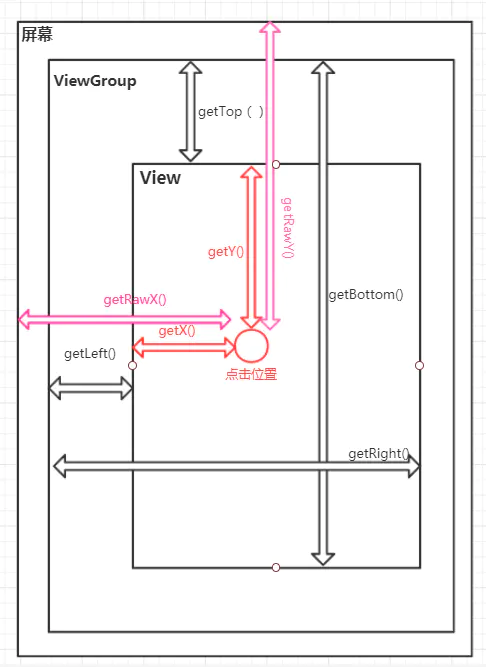
\includegraphics[width=.9\linewidth]{./pic/view.png}

\subsubsection{3. 看一下View\#layout(int l, int t, int r, int b)源码}
\label{sec-1-5-3}
\begin{minted}[frame=lines,fontsize=\scriptsize,linenos=false]{java}
public void layout(int l, int t, int r, int b) {
    if ((mPrivateFlags3 & PFLAG3_MEASURE_NEEDED_BEFORE_LAYOUT) != 0) {
        onMeasure(mOldWidthMeasureSpec, mOldHeightMeasureSpec);
        mPrivateFlags3 &= ~PFLAG3_MEASURE_NEEDED_BEFORE_LAYOUT;
    }
    int oldL = mLeft;
    int oldT = mTop;
    int oldB = mBottom;
    int oldR = mRight;
    boolean changed = isLayoutModeOptical(mParent) ?
        setOpticalFrame(l, t, r, b) : setFrame(l, t, r, b);
    if (changed || (mPrivateFlags & PFLAG_LAYOUT_REQUIRED) == PFLAG_LAYOUT_REQUIRED) {
        onLayout(changed, l, t, r, b);
        //   ....省略其它部分
    }
}
private boolean setOpticalFrame(int left, int top, int right, int bottom) {
    Insets parentInsets = mParent instanceof View ?
        ((View) mParent).getOpticalInsets() : Insets.NONE;
    Insets childInsets = getOpticalInsets();
    return setFrame(
        left   + parentInsets.left - childInsets.left,
        top    + parentInsets.top  - childInsets.top,
        right  + parentInsets.left + childInsets.right,
        bottom + parentInsets.top  + childInsets.bottom);
}
protected boolean setFrame(int left, int top, int right, int bottom) {
    boolean changed = false;
    // ....省略其它部分
    if (mLeft != left || mRight != right || mTop != top || mBottom != bottom) {
        changed = true;
        int drawn = mPrivateFlags & PFLAG_DRAWN;
        int oldWidth = mRight - mLeft;
        int oldHeight = mBottom - mTop;
        int newWidth = right - left;
        int newHeight = bottom - top;
        boolean sizeChanged = (newWidth != oldWidth) || (newHeight != oldHeight);
        invalidate(sizeChanged);
        mLeft = left;
        mTop = top;
        mRight = right;
        mBottom = bottom;
        mRenderNode.setLeftTopRightBottom(mLeft, mTop, mRight, mBottom);
        mPrivateFlags |= PFLAG_HAS_BOUNDS;
        if (sizeChanged) 
            sizeChange(newWidth, newHeight, oldWidth, oldHeight);
        if ((mViewFlags & VISIBILITY_MASK) == VISIBLE || mGhostView != null) {
            mPrivateFlags |= PFLAG_DRAWN;
            invalidate(sizeChanged);
            invalidateParentCaches();
        }
        mPrivateFlags |= drawn;
        mBackgroundSizeChanged = true;
        mDefaultFocusHighlightSizeChanged = true;
        if (mForegroundInfo != null) 
            mForegroundInfo.mBoundsChanged = true;
        notifySubtreeAccessibilityStateChangedIfNeeded();
    }
    return changed;
}
\end{minted}
\begin{itemize}
\item 四个参数l、t、r、b分别代表View的左、上、右、下四个边界相对于其父View的距离。 在调用onLayout(changed, l, t, r, b);之前都会调用到setFrame()确定View在父容器当中的位置,赋值给mLeft,mTop,mRight,mBottom。 在ViewGroup\#onLayout()跟View\#onLayout()都是空实现,交给继承者根据自身需求去定位
\item 部分零散知识点:
\begin{itemize}
\item getMeasureWidth()与getWidth() getMeasureWidth()返回的是mMeasuredWidth,而该值是在setMeasureDimension()中的setMeasureDimensionRaw()中设置的。因此onMeasure()后的所有方法都能获取到这个值。 getWidth返回的是mRight-mLeft,这两个值,是在layout()中的setFrame()中设置的. getMeasureWidthAndState中有一句: This should be used during measurement and layout calculations only. Use \{@link \#getWidth()\} to see how wide a view is after layout.
\item 总结:只有在测量过程中和布局计算时,才用getMeasuredWidth()。在layout之后,用getWidth()来获取宽度
\end{itemize}
\end{itemize}

\subsection{六、draw()绘画过程}
\label{sec-1-6}
\begin{minted}[frame=lines,fontsize=\scriptsize,linenos=false]{java}
 /*
         * Draw traversal performs several drawing steps which must be executed
         * in the appropriate order:
         *
         *      1\. Draw the background
         *      2\. If necessary, save the canvas' layers to prepare for fading
         *      3\. Draw view's content
         *      4\. Draw children
         *      5\. If necessary, draw the fading edges and restore layers
         *      6\. Draw decorations (scrollbars for instance)
         */
\end{minted}
\begin{itemize}
\item 上面是draw()里面写的绘画顺序。
\begin{itemize}
\item 绘制背景。
\item 如果必要的话,保存当前canvas
\item 绘制View的内容
\item 绘制子View
\item 如果必要的话,绘画边缘重新保存图层
\item 画装饰(例如滚动条)
\end{itemize}
\end{itemize}
\subsubsection{1. 看一下View\#draw()源码的实现}
\label{sec-1-6-1}
\begin{minted}[frame=lines,fontsize=\scriptsize,linenos=false]{java}
public void draw(Canvas canvas) {
    // Step 1, draw the background, if needed
    int saveCount;
    if (!dirtyOpaque) 
        drawBackground(canvas);

    // skip step 2 & 5 if possible (common case)

    final int viewFlags = mViewFlags;
    boolean horizontalEdges = (viewFlags & FADING_EDGE_HORIZONTAL) != 0;
    boolean verticalEdges = (viewFlags & FADING_EDGE_VERTICAL) != 0;
    if (!verticalEdges && !horizontalEdges) {
        // Step 3, draw the content
        if (!dirtyOpaque) onDraw(canvas);

        // Step 4, draw the children
        dispatchDraw(canvas);
        drawAutofilledHighlight(canvas);

        // Overlay is part of the content and draws beneath Foreground
        if (mOverlay != null && !mOverlay.isEmpty()) 
            mOverlay.getOverlayView().dispatchDraw(canvas);

        // Step 6, draw decorations (foreground, scrollbars)
        onDrawForeground(canvas);

        // Step 7, draw the default focus highlight
        drawDefaultFocusHighlight(canvas);

        if (debugDraw()) 
            debugDrawFocus(canvas);
        return;
    }
}
\end{minted}
\begin{itemize}
\item 由上面可以看到 先调用drawBackground(canvas) ->onDraw(canvas)->dispatchDraw(canvas)->onDrawForeground(canvas)越是后面绘画的越是覆盖在最上层。
\item drawBackground(canvas):画背景,不可重写
\item onDraw(canvas):画主体
\begin{itemize}
\item 代码写在super.onDraw()前:会被父类的onDraw覆盖
\item 代码写在super.onDraw()后:不会被父类的onDraw覆盖
\end{itemize}
\item dispatchDraw() :绘制子 View 的方法
\begin{itemize}
\item 代码写在super.dispatchDraw(canvas)前:把绘制代码写在 super.dispatchDraw() 的上面,这段绘制就会在 onDraw() 之后、 super.dispatchDraw() 之前发生,也就是绘制内容会出现在主体内容和子 View 之间。而这个…… 其实和重写 onDraw() 并把绘制代码写在 super.onDraw() 之后的做法,效果是一样的。
\item 代码写在super.dispatchDraw(canvas)后:只要重写 dispatchDraw(),并在 super.dispatchDraw() 的下面写上你的绘制代码,这段绘制代码就会发生在子 View 的绘制之后,从而让绘制内容盖住子 View 了。
\end{itemize}
\item onDrawForeground(canvas):包含了滑动边缘渐变和滑动条跟前景
\begin{itemize}
\item 一般来说,一个 View(或 ViewGroup)的绘制不会这几项全都包含,但必然逃不出这几项,并且一定会严格遵守这个顺序。例如通常一个 LinearLayout 只有背景和子 View,那么它会先绘制背景再绘制子 View;一个 ImageView 有主体,有可能会再加上一层半透明的前景作为遮罩,那么它的前景也会在主体之后进行绘制。需要注意,前景的支持是在 Android 6.0(也就是 API 23)才加入的;之前其实也有,不过只支持 FrameLayout,而直到 6.0 才把这个支持放进了 View 类里。
\end{itemize}
\end{itemize}

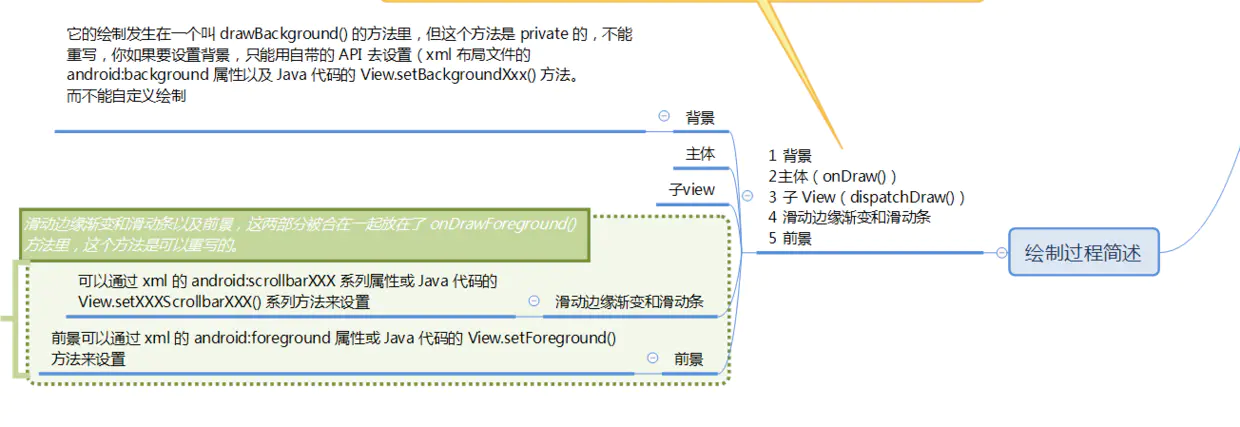
\includegraphics[width=.9\linewidth]{./pic/drawprocess.png}

\subsubsection{2. 注意事项}
\label{sec-1-6-2}
\begin{enumerate}
\item 2.1 在 ViewGroup 的子类中重写除 dispatchDraw() 以外的绘制方法时,可能需要调用 setWillNotDraw(false);
\label{sec-1-6-2-1}
\begin{itemize}
\item 出于效率的考虑,ViewGroup 默认会绕过 draw() 方法,换而直接执行 dispatchDraw(),以此来简化绘制流程。所以如果你自定义了某个 ViewGroup 的子类(比如 LinearLayout)并且需要在它的除 dispatchDraw() 以外的任何一个绘制方法内绘制内容,你可能会需要调用 View.setWillNotDraw(false) 这行代码来切换到完整的绘制流程(是「可能」而不是「必须」的原因是,有些 ViewGroup 是已经调用过 setWillNotDraw(false) 了的,例如 ScrollView)。
\end{itemize}
\item 2.2 在重写的方法有多个选择时,优先选择 onDraw()
\label{sec-1-6-2-2}
\begin{itemize}
\item 一段绘制代码写在不同的绘制方法中效果是一样的,这时你可以选一个自己喜欢或者习惯的绘制方法来重写。但有一个例外:如果绘制代码既可以写在 onDraw() 里,也可以写在其他绘制方法里,那么优先写在 onDraw() ,因为 Android 有相关的优化,可以在不需要重绘的时候自动跳过 onDraw() 的重复执行,以提升开发效率。享受这种优化的只有 onDraw() 一个方法。
\end{itemize}
\end{enumerate}
\subsection{七、在Activity中获取View的宽高的几种方式}
\label{sec-1-7}
\begin{itemize}
\item Activity 获取 view 的宽高, 在 onCreate , onResume 等方法中获取到的都是0, 因为 View 的测量过程并不是和 Activity 的声明周期同步执行的
\end{itemize}
\subsubsection{1. view.post}
\label{sec-1-7-1}
\begin{itemize}
\item post 可以将一个 runnable 投递到消息队列的尾部,然后等待 Looper 调用此 runnable 的时候, View 也已经初始化好了
\begin{minted}[frame=lines,fontsize=\scriptsize,linenos=false]{java}
view.post(new Runnable() {
    @Override
    public void run() {
        int width = view.getMeasuredWidth();
        int height = view.getMeasuredHeight(); 
    }
});
\end{minted}
\end{itemize}
\subsubsection{2. ViewTreeObserver}
\label{sec-1-7-2}
\begin{itemize}
\item 使用 addOnGlobalLayoutListener 接口, 当 view 树的状态发生改变或者 View 树内部的 view 的可见性发生改变时, onGlobalLayout() 都会被调用, 需要注意的是, onGlobalLayout 方法可能被调用多次, 代码如下:
\begin{minted}[frame=lines,fontsize=\scriptsize,linenos=false]{java}
 view.getViewTreeObserver().addOnGlobalLayoutListener(new ViewTreeObserver.OnGlobalLayoutListener() {
            @Override
            public void onGlobalLayout() {
                view.getViewTreeObserver().removeOnGlobalLayoutListener(this);
                int width = view.getMeasuredWidth();
                int height = view.getMeasuredHeight();
            }
        });
\end{minted}
\end{itemize}
\subsubsection{3. onWindowFocusChanged}
\label{sec-1-7-3}
\begin{itemize}
\item 这个方法的含义是 View 已经初始化完毕了, 宽高已经准备好了, 需要注意的就是这个方法可能会调用多次, 在 Activity onResume 和onPause的时候都会调用, 也会有多次调用的情况
\begin{minted}[frame=lines,fontsize=\scriptsize,linenos=false]{java}
 @Override
public void onWindowFocusChanged(boolean hasWindowFocus) {
    super.onWindowFocusChanged(hasWindowFocus);
    if (hasWindowFocus){
        int width = view.getMeasuredWidth();
        int height = view.getMeasuredHeight();
    }
}
\end{minted}
\end{itemize}


\subsection{View 工作流程}
\label{sec-1-8}
\begin{itemize}
\item 通过 SetContentView(),调用 到PhoneWindow ,后实例DecorView ,通过 LoadXmlResourceParser() 进行IO操作 解析xml文件 通过反射 创建出View,并将View绘制在 DecorView上,这里的绘制则交给了ViewRootImpl 来完成,通过performTraversals() 触发绘制流程,performMeasure 方法获取View的尺寸,performLayout 方法获取View的位置 ,然后通过 performDraw 方法遍历View 进行绘制。
\end{itemize}
\subsection{事件分发}
\label{sec-1-9}
\begin{itemize}
\item 一个 MotionEvent 产生后,按 Activity -> Window -> DecorView(ViewGroup) -> View 顺序传递,View 传递过程就是事件分发,因为开发过程中存在事件冲突,所以需要熟悉流程:
\begin{itemize}
\item dispatchTouchEvent:用于分发事件,只要接受到点击事件就会被调用,返回结果表示是否消耗了当前事件
\item onInterceptTouchEvent:用于判断是否拦截事件(只有ViewGroup中存在),当 ViewGroup 确定要拦截事件后,该事件序列都不会再触发调用此 ViewGroup 的 onIntercept
\item onTouchEvent:用于处理事件,返回结果表示是否处理了当前事件,未处理则传递给父容器处理。(事件顺序是:OnTouchListener -> OnTouchEvent -> OnClick)
\end{itemize}
\end{itemize}
\subsection{自定义View!!}
\label{sec-1-10}
准备自定义View方面的面试最简单的方法:

就是自己动手实现几个View(由简单到复杂);
分析一些热门App中的自定义View的效果是怎么实现的;
阿里面试官: 自定义View跟绘制流程相关知识点?(标准参考解答,值得收藏)
\begin{itemize}
\item \url{https://www.cnblogs.com/Android-Alvin/p/12297933.html}
\end{itemize}
% Emacs 27.1 (Org mode 8.2.7c)
\end{document}